\section{Kamil Pustelnik}
\label{sec:kpust}

Twierdzenie Pitagorasa: $a^2 + b^2 = c^2$
Wzór na pole koła: \[(p - x)^2 + (q - y)^2 \leq r^2\]

Czy widzieliście już pociąg Pendolino (Figure~\ref{fig:pendolino})?
Alternatywnie warto zobaczyć również przeciętny pociąg PKP (Figure~\ref{fig:pociag_pkp}).
Wyglądają o wiele lepiej niż np. pociągi \href{https://kolejemalopolskie.com.pl/}{Kolei Małopolskich} (Figure~\ref{fig:pociag_kmp}).

\begin{figure}[htbp]
    \centering
    \label{fig:pendolino}
    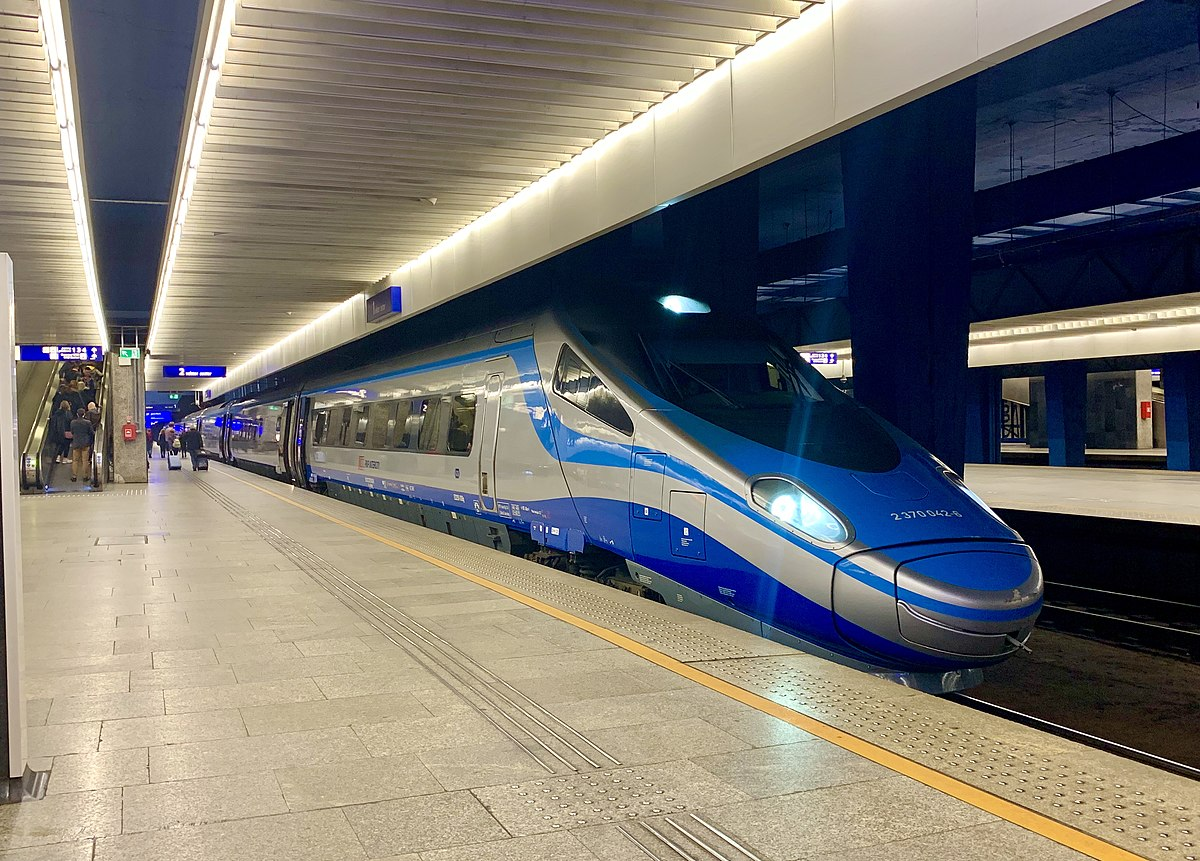
\includegraphics[width=0.5\textwidth]{pictures/Pendolino.jpg}
    \caption{PKP Pendolino na Warszawskiej stacji kolejowej}
\end{figure}

\begin{figure}[htbp]
    \centering
    \label{fig:pociag_pkp}
    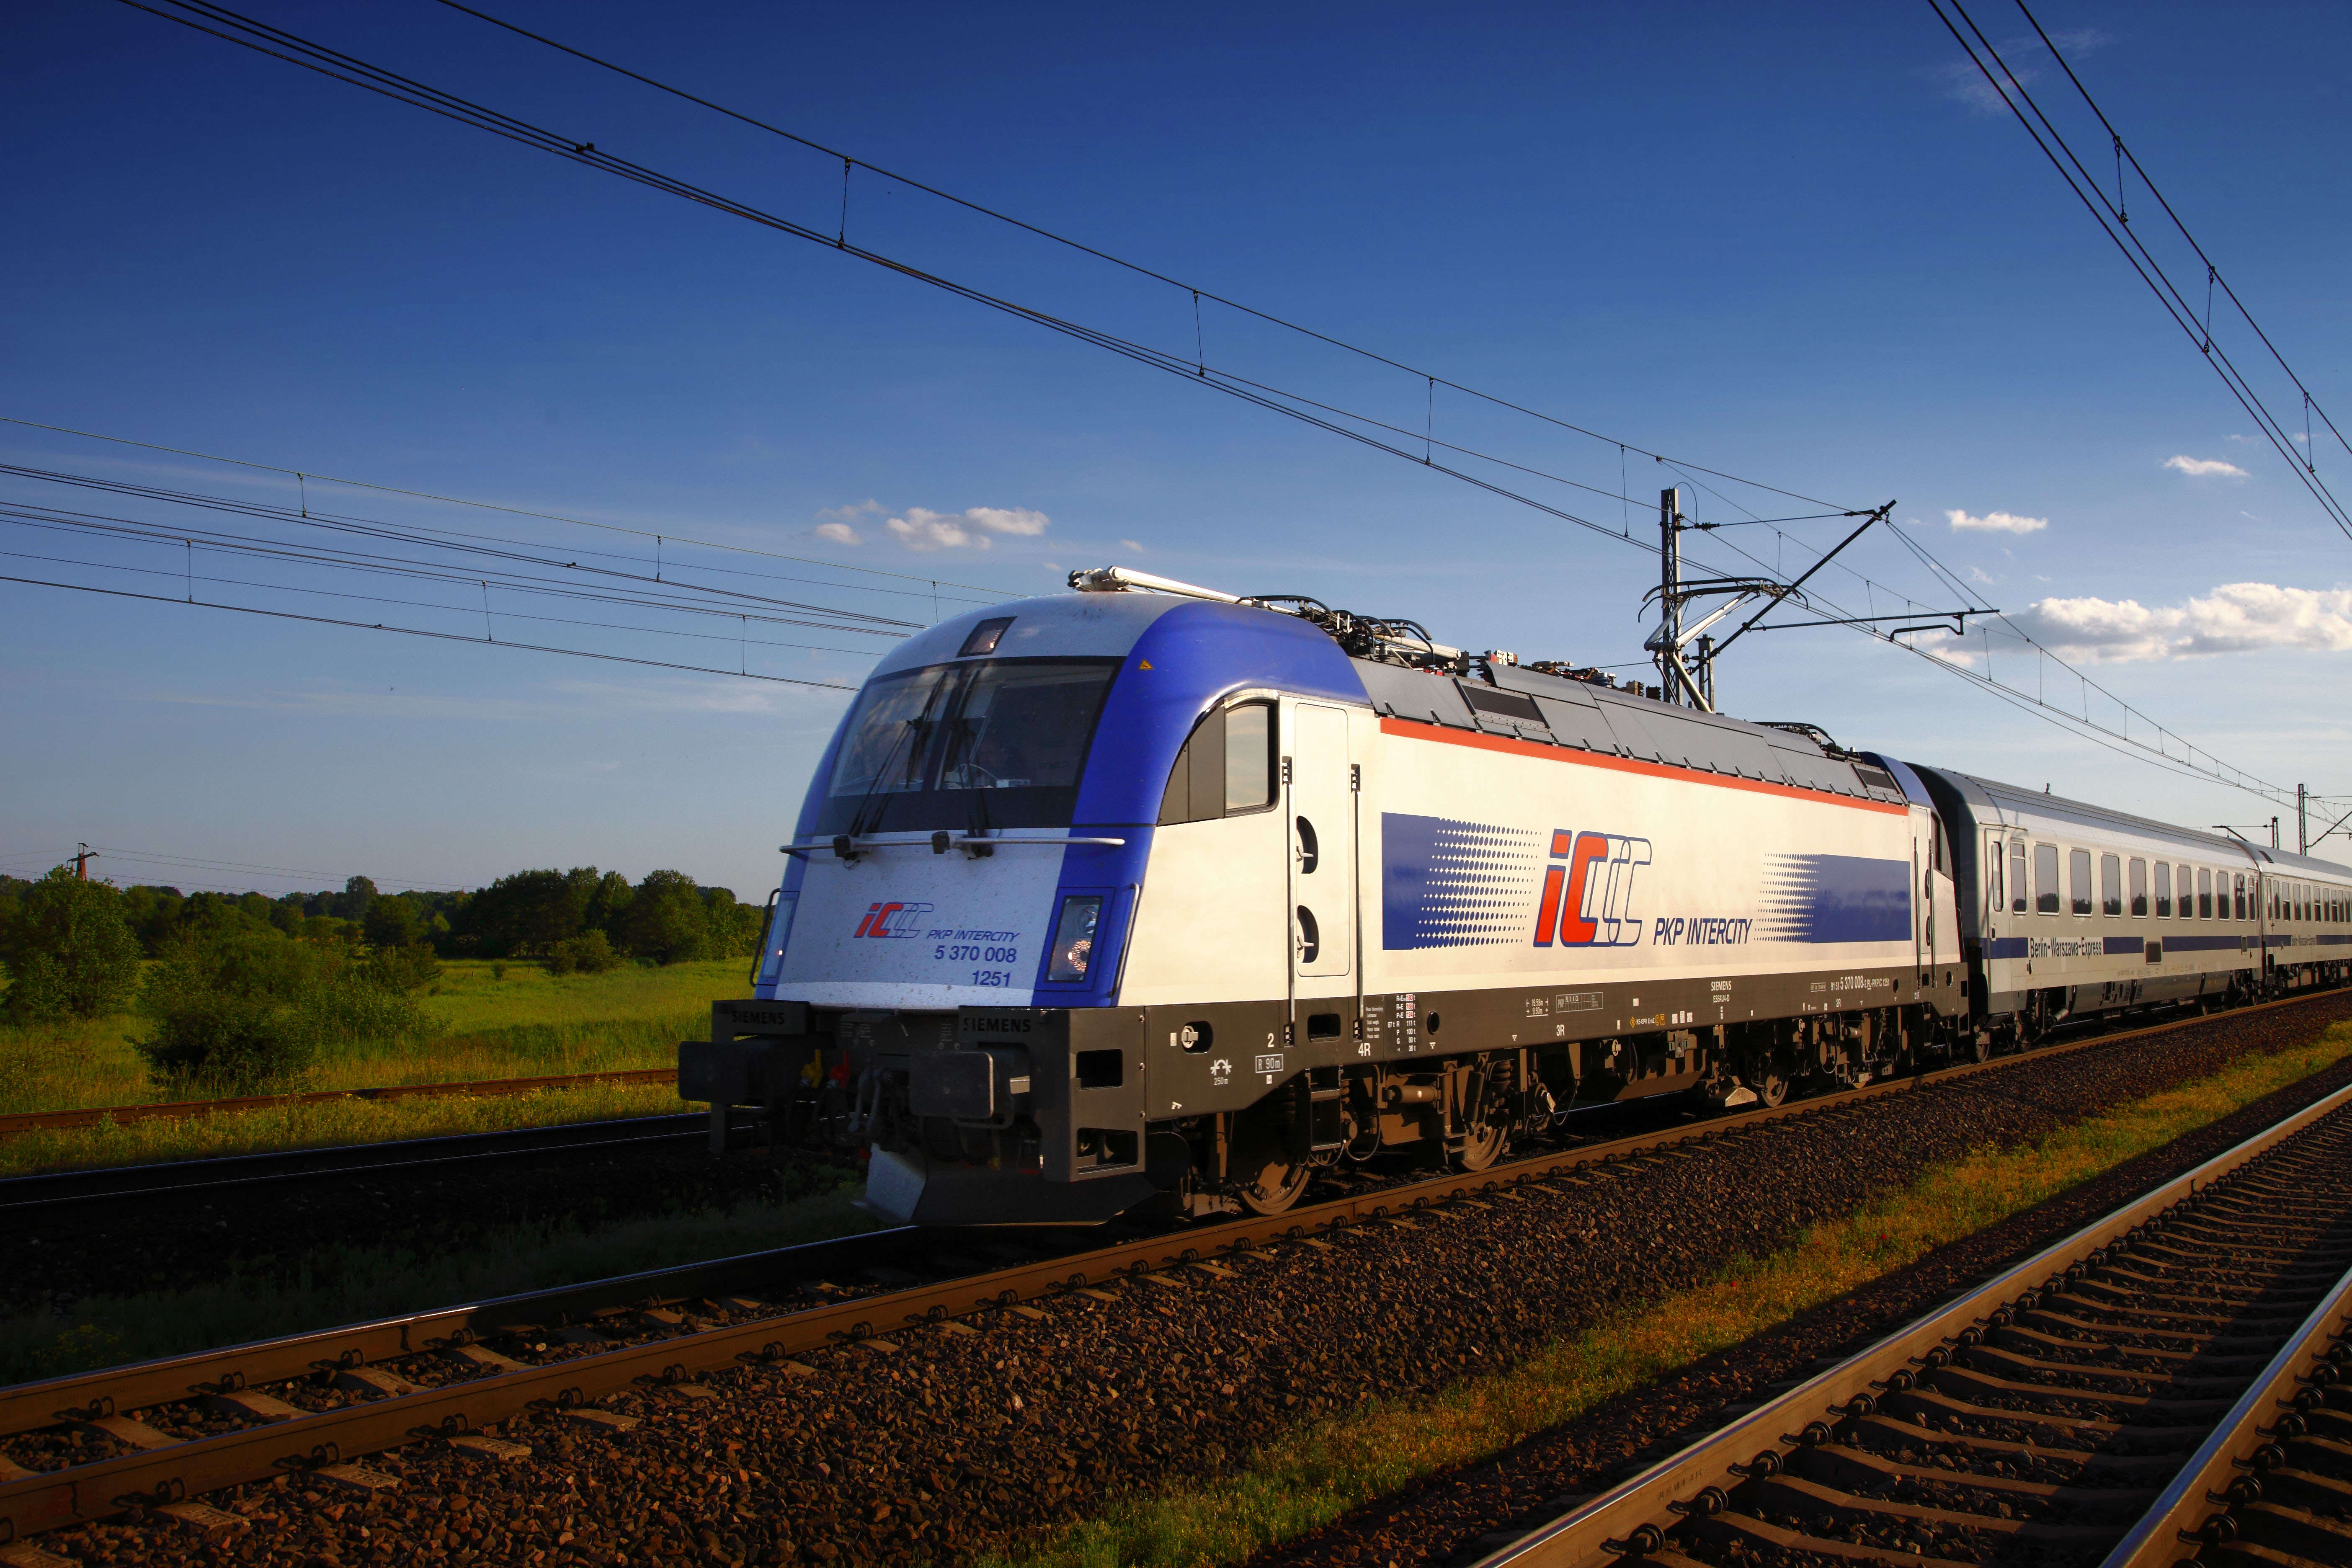
\includegraphics[width=0.5\textwidth]{pictures/pociag_pkp.jpg}
    \caption{Przeciętny pociąg PKP}
\end{figure}

\begin{figure}[htbp]
    \centering
    \label{fig:pociag_kmp}
    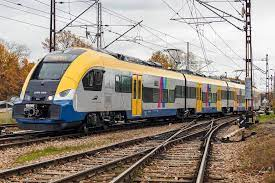
\includegraphics[width=0.5\textwidth]{pictures/pociag_KMP.jpeg}
    \caption{Przykładowy pociąg Kolei Małopolskich}
\end{figure}

Parę faktów o pociągach typu \emph{Pendolino}:
\begin{itemize}
    \item Są szybkie!
    \item Są drogie!
    \item Często się spóźniają.
\end{itemize}

Aby zakupić bilet należy:
\begin{enumerate}
    \item Wejść na stronę \url{https://www.intercity.pl/}
    \item Wybrać stację początkową i końcowa
    \item Wybrać dzień podróży
    \item Zatwierdzić wybór
    \item Liczyć, że strona PKP zadziała\footnote{W trakcie pisania tego tekstu (\date{25.10.2023}) strona nie działała poprawnie - po wyszukaniu pociągów wyświetlał się komunikat \emph{Bad request}.}
\end{enumerate}

Dlatego:
\begin{itemize}
    \item[?] Warto rozważyć innego przewoźnika.
    \item[!] Nie ufaj PKP!
    \item[*] nigdy
\end{itemize}

Niewarto zatem jest ufać pociągom PKP, ponieważ często okazują się \emph{niegodne} tego zaufania. Warto rozważyć wybór innych przewoźników lub alternatywnej formy transportu.\par
A jeżeli wszystkie opcje zawiodą, może warto przesiąść się na \underline{rower}? Jeżeli pomimo wszystko konieczne będzie użycie pociągu \textbf{PKP}, to warto zapoznać się z tabelą pociągów, w których konieczna jest \underline{\textit{rezerwacja miejsc}}. Część tej tabeli znajduje się poniżej. Tabela~\ref{tab:pociagi} przedstawia pociągi objęte obowiązkową rezerwacją miejsc (niektóre to pociągi pendolino takie jak na rysunku~\ref{fig:pendolino} ze strony \pageref{fig:pendolino}). Pełną listę można znaleźć \href{https://www.intercity.pl/pl/site/o-nas/dzial-prasowy/komunikaty/lista-pociagow-objetych-obowiazkowa-rezerwacja-miejsc.html}{na tej stronie internetowej}.

\begin{table}[htbp]
\centering
\begin{tabular}{|llllll|}
\hline
\textbf{l.p.}           & \textbf{Kategoria}      & \textbf{Nr poc.}            & \textbf{Nazwa poc.}            & \textbf{Stacja od}                               & \textbf{Stacja do}          \\ \hline
\multicolumn{1}{|l|}{1} & \multicolumn{1}{l|}{IC} & \multicolumn{1}{l|}{6120/1} & \multicolumn{1}{l|}{ASNYK}     & \multicolumn{1}{l|}{Wrocław Główny}              & \textit{Warszawa Gdańska}   \\ \hline
\multicolumn{1}{|l|}{2} & \multicolumn{1}{l|}{IC} & \multicolumn{1}{l|}{1620/1} & \multicolumn{1}{l|}{ASNYK}     & \multicolumn{1}{l|}{\textit{Warszawa Wschodnia}} & Wrocław Główny              \\ \hline
\multicolumn{1}{|l|}{3} & \multicolumn{1}{l|}{IC} & \multicolumn{1}{l|}{6122/3} & \multicolumn{1}{l|}{BACZYŃSKI} & \multicolumn{1}{l|}{Wrocław Główny}              & \textit{Warszawa Wschodnia} \\ \hline
\multicolumn{1}{|l|}{4} & \multicolumn{1}{l|}{IC} & \multicolumn{1}{l|}{2622/3} & \multicolumn{1}{l|}{BACZYŃSKI} & \multicolumn{1}{l|}{Lublin Główny}               & Wrocław Główny              \\ \hline
\multicolumn{1}{|l|}{5} & \multicolumn{1}{l|}{IC} & \multicolumn{1}{l|}{1622/3} & \multicolumn{1}{l|}{BACZYŃSKI} & \multicolumn{1}{l|}{\textit{Warszawa Gdańska}}   & Wrocław Główny              \\ \hline
\multicolumn{1}{|l|}{6} & \multicolumn{1}{l|}{IC} & \multicolumn{1}{l|}{5700/1} & \multicolumn{1}{l|}{BAŁTYK}    & \multicolumn{1}{l|}{Gdynia Główna}               & Poznań Główny               \\ \hline
\multicolumn{1}{|l|}{7} & \multicolumn{1}{l|}{IC} & \multicolumn{1}{l|}{7500/1} & \multicolumn{1}{l|}{BAŁTYK}    & \multicolumn{1}{l|}{Poznań Główny}               & Gdynia Główna               \\ \hline
\multicolumn{1}{|l|}{8} & \multicolumn{1}{l|}{IC} & \multicolumn{1}{l|}{7322/3} & \multicolumn{1}{l|}{BARBAKAN}  & \multicolumn{1}{l|}{Poznań Główny}               & {\ul Kraków Główny}         \\ \hline
\multicolumn{1}{|l|}{9} & \multicolumn{1}{l|}{IC} & \multicolumn{1}{l|}{3722/3} & \multicolumn{1}{l|}{BARBAKAN}  & \multicolumn{1}{l|}{{\ul Kraków Główny}}         & Poznań Główny               \\ \hline
\end{tabular}
\label{tab:pociagi}
\caption{Pociągi, w których obowiązuje obowiązkowa rezerwacja miejsc}
\end{table}
